\chapter{3D Printer}

\section{Binder Jetting}
In Binder Jetting, A roller or blade spreads a fresh, even layer of part material powder over the build surface. The print head \textbf{selectively sprays the binder} onto specific regions of the powder bed, as defined by the 3D model. The \textbf{binder fuses the powder particles together} to form solid layers of the desired part geometry. The build \textbf{platform lowers incrementally}, and the process repeats until the part is complete.

{\begin{wrapfigure}{r}{0.4\textwidth}
   \centering
   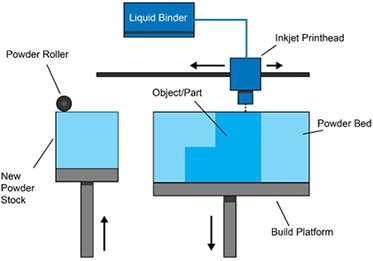
\includegraphics[width=\linewidth]{figures/Binder Jetting.jpg}
\end{wrapfigure}
\textbf{Post-Processing:}
\vspace{-0.65\baselineskip}
\begin{itemize}[parsep=0.25em]
   \item \textit{\textbf{Depowdering}:} to remove the excess powder.
   \item \textit{\textbf{Sintering \& Infiltration}:} to improve appearance and durability.
\end{itemize}}

\textbf{Key Features:}
\vspace{-0.65\baselineskip}
\begin{itemize}[parsep=0.25em]
   \item \rgbO{No supports needed} (powder supports overhangs).
   \item Works with metals, ceramics, sand, and polymers.
   \item Faster and more \rgbO{cost-effective} than laser-based powder-bed methods.
\end{itemize}

\textbf{Limitations:}
\vspace{-0.65\baselineskip}
\begin{itemize}[parsep=0.25em]
   \item Lower mechanical strength compared to lased based AM.
   \item Rougher surface finish compared to other methods.
   \item Require additional post-processing for strength and finish.
\end{itemize}

% \vspace{2em}
% Alternatively:
% \begin{itemize}[parsep=0.5em]
%    \item \textbf{Powder Layering:} A roller or blade spreads a fresh, even layer of part material powder over the build surface.
   
%    \item \textbf{Binder Jetting:} The print head selectively sprays the binder onto specific regions of the powder bed, as defined by the 3D model.
   
%    \item \textbf{Layer Stacking:} The build platform lowers incrementally, and the process repeats until the part is complete.
   
%    \item \textbf{Post-Processing:} Excess powder is removed, and parts are cured/sintered for strength.
%    \begin{itemize}[parsep=0.5em]
%       \item \textit{\textbf{Depowdering}:} to remove the excess powder.
%       \item \textit{\textbf{Sintering \& Infiltration}:} to improve appearance and durability.
%    \end{itemize}
% \end{itemize}

\section{Material Jetting}
In Material Jetting, droplets of actual build materials typically liquid photopolymers or resins are deposited directly  onto the build platform through multiple print heads. Each deposited layer is then instantly cured (hardened) using a UV light, ensuring dimensional stability. Support materials are jetted alongside and later removed once finished.

{\begin{wrapfigure}{r}{0.3\textwidth}
   \vspace{-1em}
   \centering
   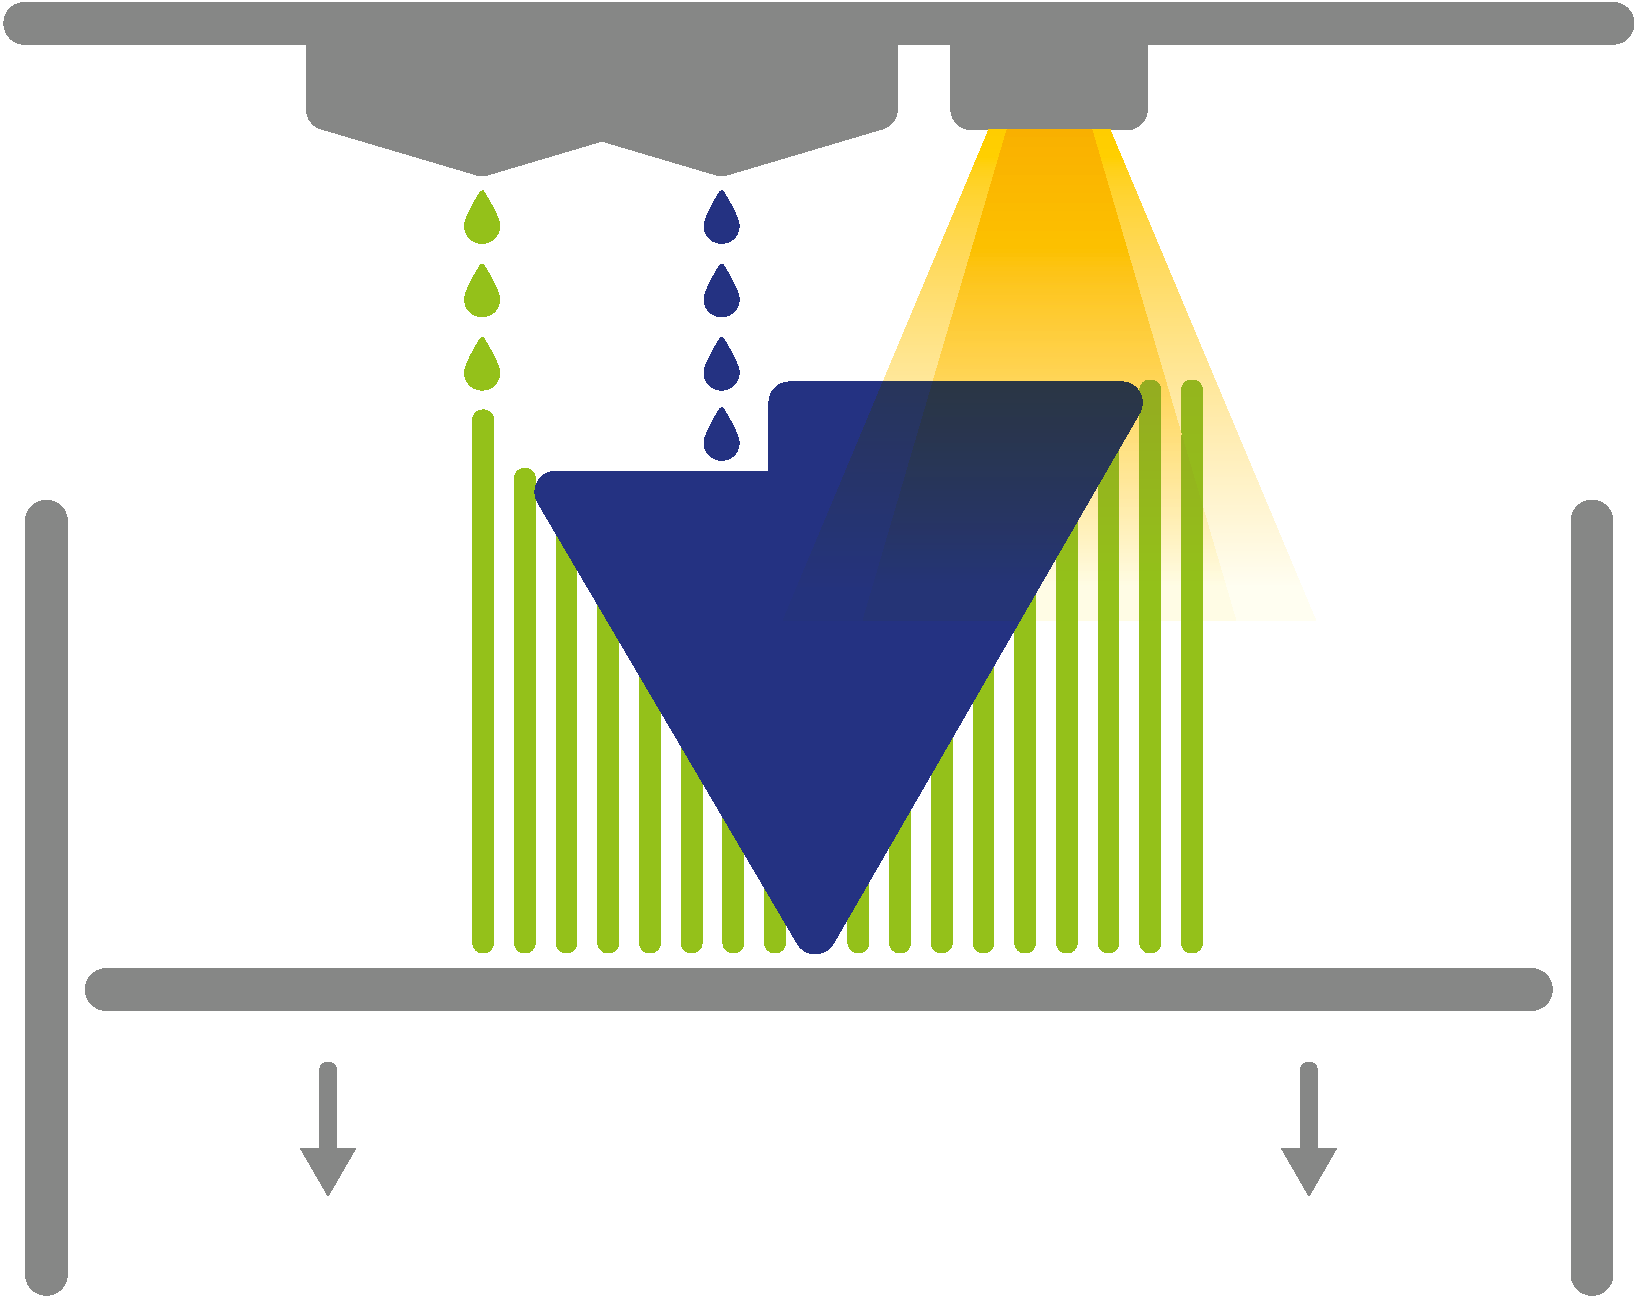
\includegraphics[width=\linewidth]{figures/Material Jetting.png}
\end{wrapfigure}
\textbf{Key Features:}
\vspace{-0.65\baselineskip}
\begin{itemize}[parsep=0.25em]
   \item Produces highly accurate parts with excellent smoothness.
   \item Allows multi-material printing of different properties in a single part.
   \item Simultaneous deposition of multiple materials reduces print time.
\end{itemize}

\textbf{Limitations:}
\vspace{-0.65\baselineskip}
\begin{itemize}[parsep=0.25em]
   \item Primarily limited to photopolymer resins which is quite expensive.
   \item Material properties degrade under UV exposure over time.
   \item Support removal can be tedious for intricate designs.
\end{itemize}}


\section{Stereolithography}
Stereolithography (SL) is a laser-based 3D printing process that uses photopolymer resin and cure to form a solid in a very precise way to produce very accurate parts. The photopolymer resin is held in a vat with a movable platform inside. A laser beam is directed in the X-Y axes across the surface of the resin according to the 3D data supplied to the machine (the .stl file), whereby the resin hardens precisely where the laser hits the surface.

{\begin{wrapfigure}{r}{0.33\textwidth}
   \vspace{-1em}
   \centering
   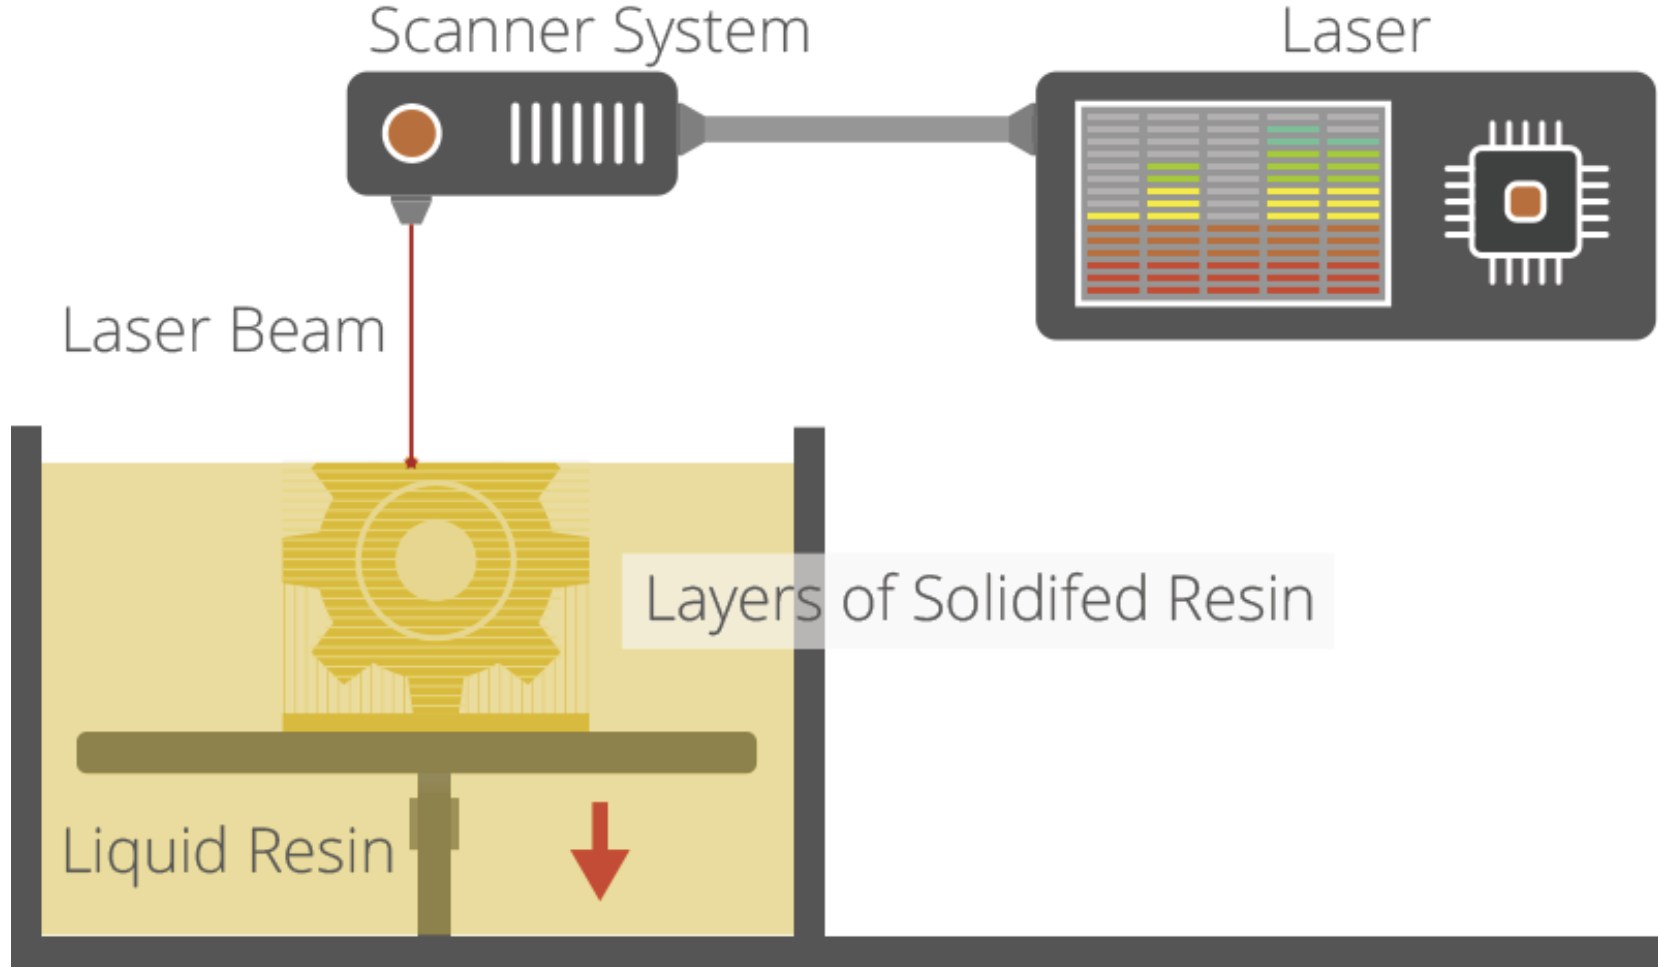
\includegraphics[width=\linewidth]{figures/Stereolithography.png}
\end{wrapfigure}\textbf{Key Features:}
\vspace{-0.65\baselineskip}
\begin{itemize}[parsep=0.25em]
   \item Excellent dimensional precision and resolution.
   \item Smooth surface finish and ideal for visual prototypes: dental, jewelry.
\end{itemize}

\textbf{Limitations:}
\vspace{-0.65\baselineskip}
\begin{itemize}[parsep=0.25em]
   \item Photopolymers degrade or brittle under UV exposure over time.
   \item Vat size restricts part dimensions and resins are expensive.
   \item Support removal can be tedious for intricate designs.
\end{itemize}}

\section{Fused Deposition Modeling (FDM)}
The thermoplastic filament is fed into a heated print head, which moves in the X and Y axes, laying down the melted material according to the 3D model data supplied to the machine. Once a layer is complete, the build platform lowers slightly along the Z-axis, and the next layer is deposited directly on top of the previous one. Each layer hardens as it is deposited and bonds to the previous layer.

{\begin{wrapfigure}{r}{0.4\textwidth}
   \vspace{-1em}
   \centering
   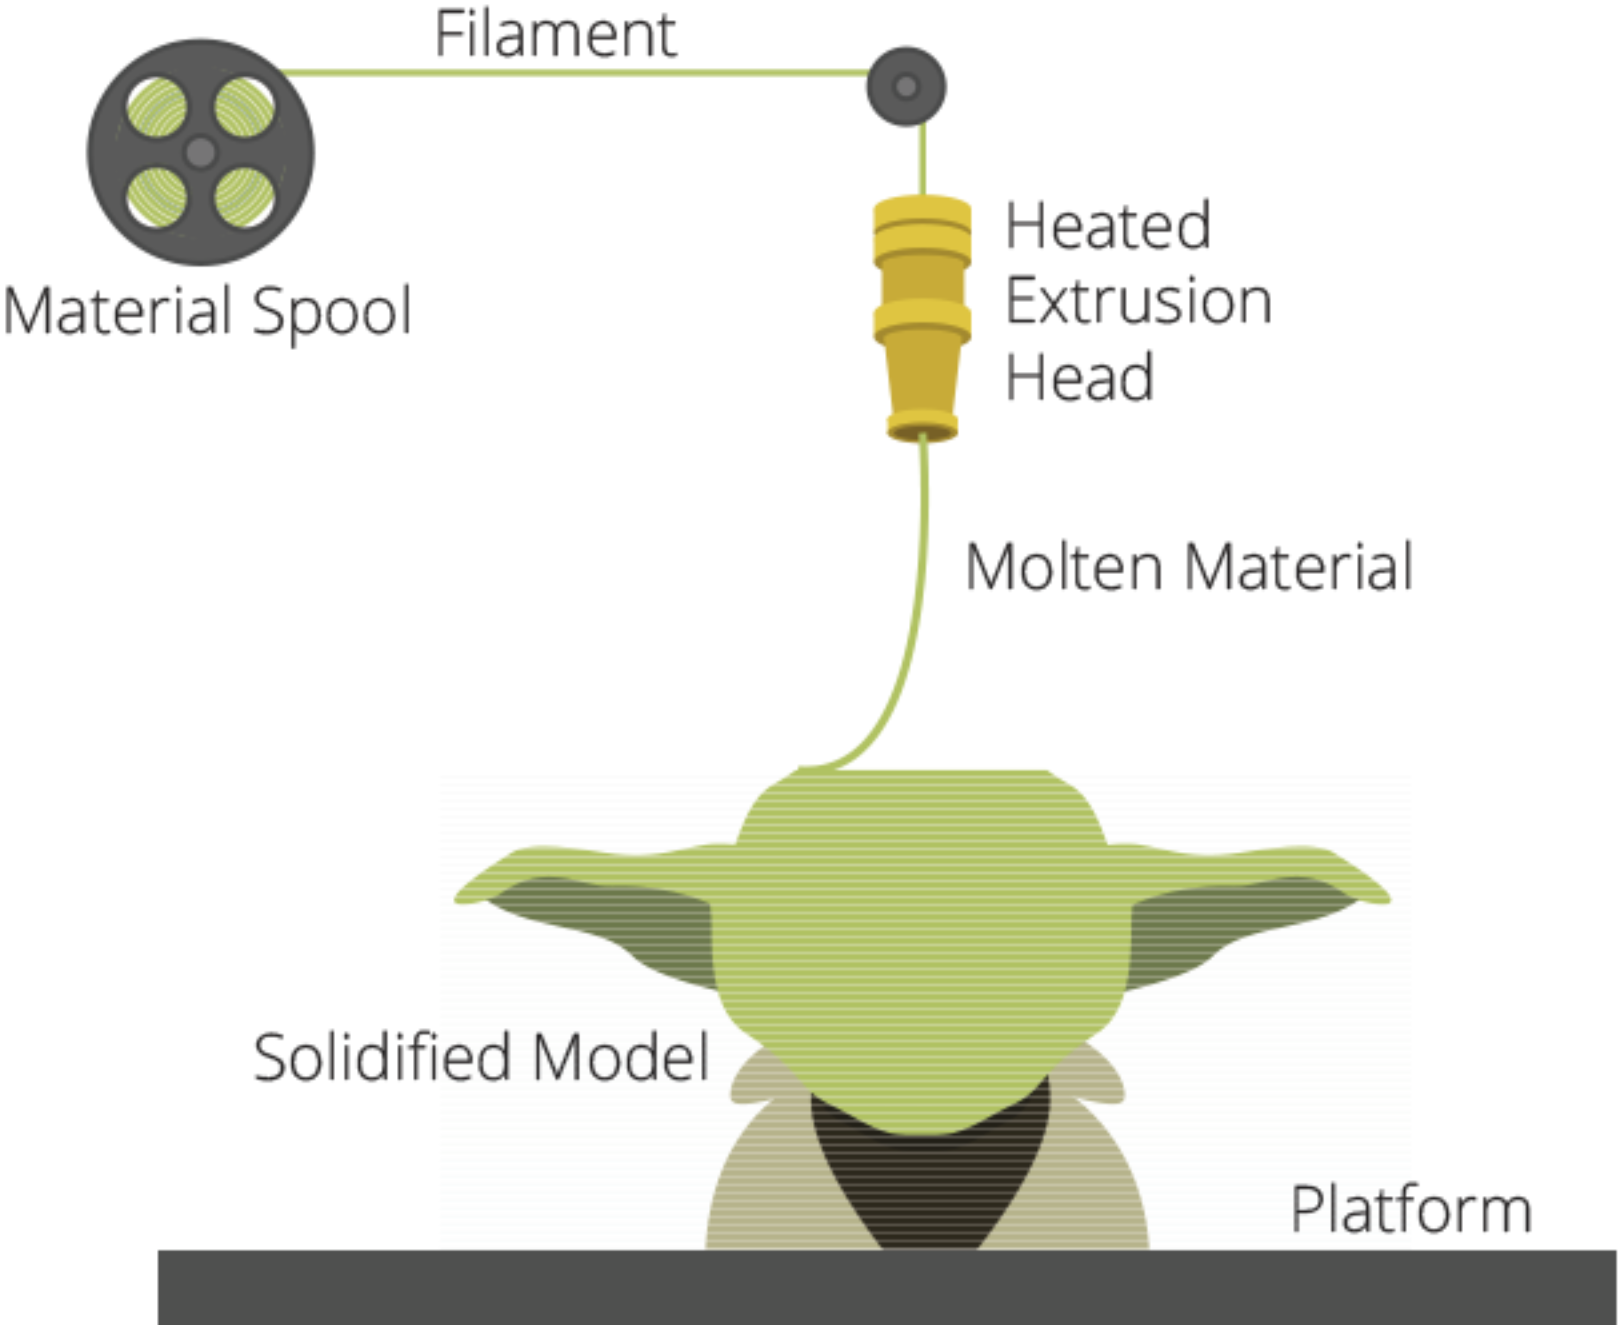
\includegraphics[width=\linewidth]{figures/FDM.png}
\end{wrapfigure}
\textbf{Key Features:}
\vspace{-0.65\baselineskip}
\begin{itemize}[parsep=0.25em]
   \item  Uses materials like PLA, ABS, Nylon;\\suitable for both prototyping and functional parts.
   \item Can use breakaway or water-soluble support materials for complex geometries.
   \item One of the most affordable and accessible 3D printing methods.
\end{itemize}

\textbf{Limitations:}
\vspace{-0.65\baselineskip}
\begin{itemize}[parsep=0.25em]
   \item  The process can be slow for some part geometries.
   \item Layer-to-layer adhesion can be a problem, resulting in parts that are not watertight.
   \item Requires post-processing using Acetone to resolve the issue.
\end{itemize}}